\documentclass{beamer}
 
\usepackage[utf8]{inputenc}
\usepackage{amsmath}
\usepackage{tabto}
\usepackage{graphicx}

 
%Information to be included in the title page:

\usetheme{Copenhagen}
\title[ADAM] %optional
{ADAM : A Method for Stochastic Optimization \\ in ICLR 2015 \\ By Diederik P. Kingma \hspace{1cm} Jimmy Lei Ba}
 
 
\author[Anshika,Razat] % (optional, for multiple authors)
{Anshika Chaurasia \and \\Razat Shanker}
 
\institute[VFU] % (optional)
{
  
  EE18MTECH11017\\
  EE18MTECH11016
 
 }
 
\date[VLC 2013] % (optional)
{14 Mar 2019}
 

\begin{document}
 
\frame{\titlepage}

\begin{frame}{Architecture}
    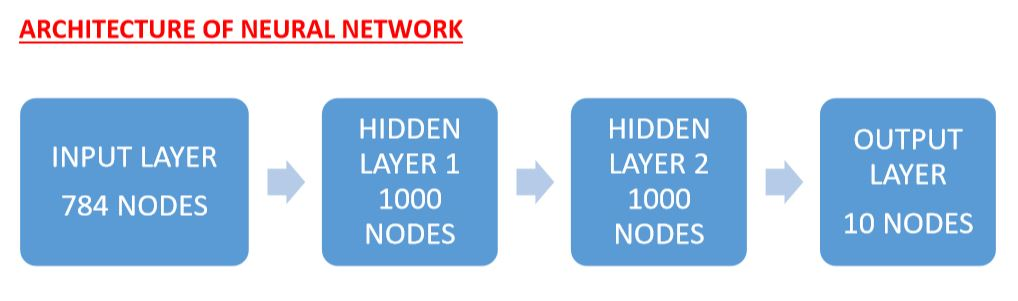
\includegraphics[width=11cm,height=5cm,angle=0]{architecture}
\end{frame}

\begin{frame}{SGD with Momentum}
 \begin{columns}
    \begin{column}{0.5\textwidth}
          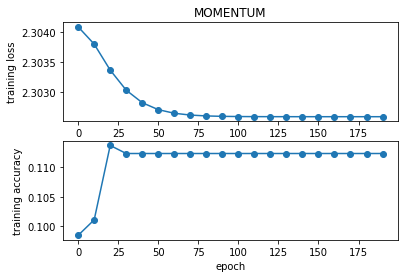
\includegraphics[width=5.5cm,height=5cm,angle=0]{mom_mini.png}\\
          \centering
          without mini-batch
    \end{column}
    \begin{column}{0.5\textwidth}
          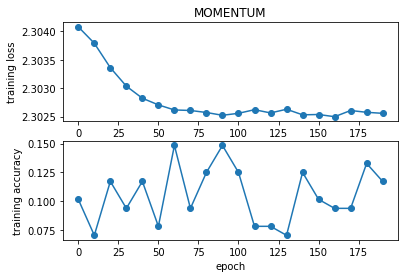
\includegraphics[width=5.5cm,height=5cm,angle=0]{mom.png}\\
          \centering
          with mini-batch
    \end{column}
 \end{columns}
\end{frame}

\begin{frame}{Nesterov}
 \begin{columns}
    \begin{column}{0.47\textwidth}
          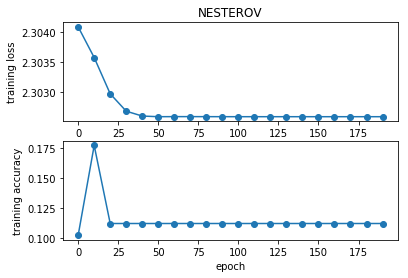
\includegraphics[width=5cm,height=5cm,angle=0]{nes_mini.png}\\
          \centering
          without mini-batch
    \end{column}
    \begin{column}{0.47\textwidth}
          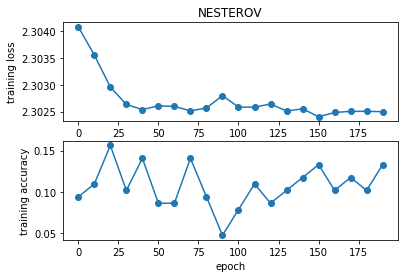
\includegraphics[width=5cm,height=5cm,angle=0]{nes.png}\\
          \centering
          with mini-batch
    \end{column}
 \end{columns}
\end{frame}


\begin{frame}{ADAGrad}
 \begin{columns}
    \begin{column}{0.47\textwidth}
          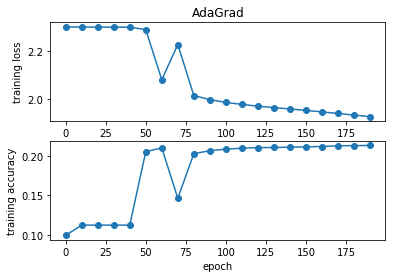
\includegraphics[width=5cm,height=5cm,angle=0]{adagrad_mini.png}\\
          \centering
          without mini-batch
    \end{column}
    \begin{column}{0.47\textwidth}
          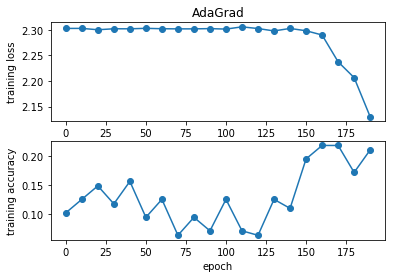
\includegraphics[width=5cm,height=5cm,angle=0]{adagrad.png}\\
          \centering
          with mini-batch
    \end{column}
 \end{columns}
\end{frame}

\begin{frame}{RMSProp}
 \begin{columns}
    \begin{column}{0.47\textwidth}
          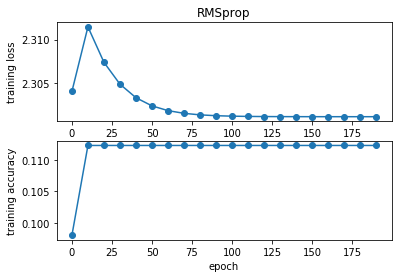
\includegraphics[width=5cm,height=5cm,angle=0]{rms_mini.png}\\
          \centering
          without mini-batch
    \end{column}
    \begin{column}{0.47\textwidth}
          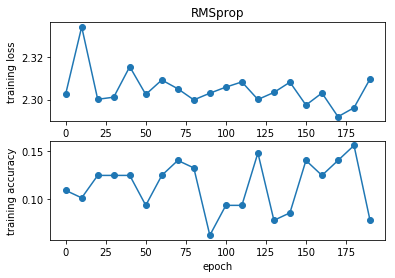
\includegraphics[width=5cm,height=5cm,angle=0]{rms.png}\\
          \centering
          with mini-batch
    \end{column}
 \end{columns}
\end{frame}

\begin{frame}{ADAM}
 \begin{columns}
    \begin{column}{0.47\textwidth}
          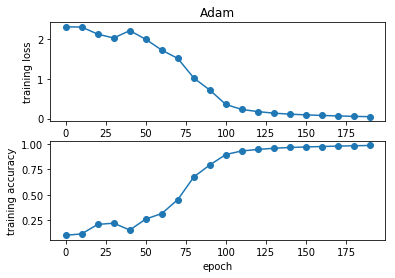
\includegraphics[width=5cm,height=5cm,angle=0]{adam_mini.png}\\
          \centering
          without mini-batch
    \end{column}
    \begin{column}{0.47\textwidth}
          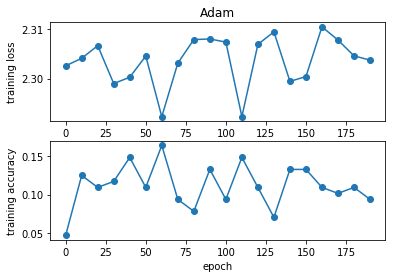
\includegraphics[width=5cm,height=5cm,angle=0]{adam.png}\\
          \centering
          with mini-batch
    \end{column}
 \end{columns}
\end{frame}

\begin{frame}{Comparison}
 \begin{columns}
    \begin{column}{0.47\textwidth}
          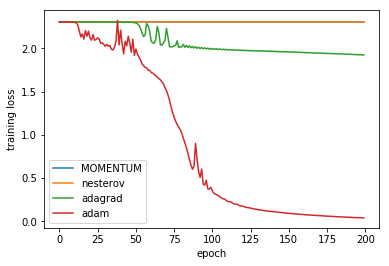
\includegraphics[width=5cm,height=5cm,angle=0]{mix_mini.png}\\
          \centering
          without mini-batch
    \end{column}
    \begin{column}{0.47\textwidth}
          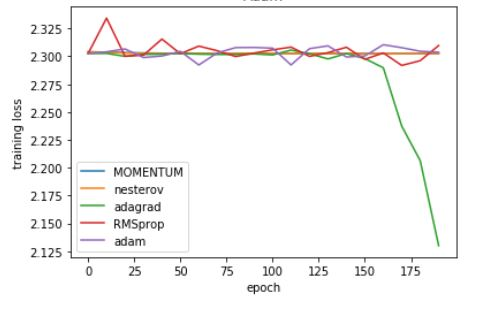
\includegraphics[width=5cm,height=5cm,angle=0]{mix.png}\\
          \centering
          with mini-batch
    \end{column}
 \end{columns}
\end{frame}
\end{document}